
\begin{figure}
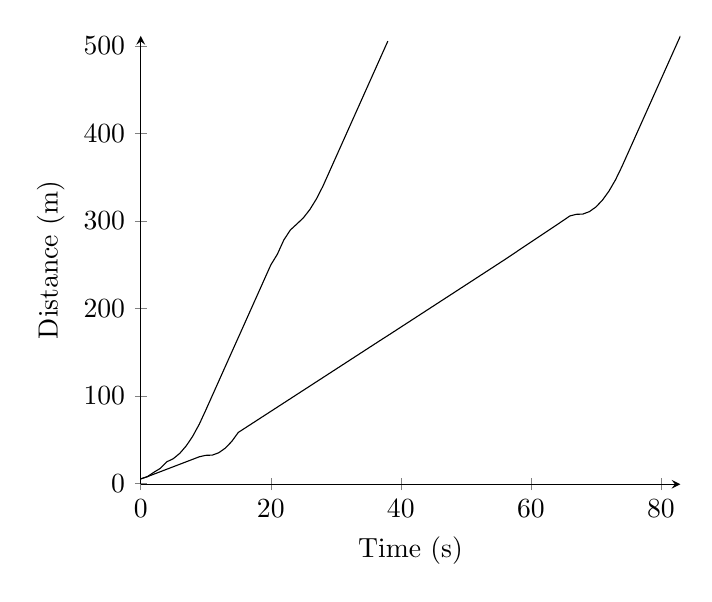
\begin{tikzpicture}
\begin{axis}[
legend style={anchor=west},
axis x line=bottom,
axis y line=left,
ymin=-1,
xlabel=Time (s),
ylabel=Distance (m),
]
\addplot[] coordinates {
(0, 5.1)
(1, 7.6)
(2, 12.6)
(3, 17.1)
(4, 24.5922199804)
(5, 28.1908323924)
(6, 34.2894448043)
(7, 42.8880572163)
(8, 53.9866696282)
(9, 67.5852820402)
(10, 83.6838944522)
(11, 100.283894452)
(12, 116.883894452)
(13, 133.483894452)
(14, 150.083894452)
(15, 166.583894452)
(16, 183.183894452)
(17, 199.783894452)
(18, 216.383894452)
(19, 232.983894452)
(20, 249.583894452)
(21, 261.723894452)
(22, 278.05220085)
(23, 289.447993151)
(24, 296.326816164)
(25, 303.326747165)
(26, 312.826678166)
(27, 324.826609167)
(28, 339.326540168)
(29, 355.926540168)
(30, 372.526540168)
(31, 389.126540168)
(32, 405.726540168)
(33, 422.326540168)
(34, 438.926540168)
(35, 455.526540168)
(36, 472.126540168)
(37, 488.726540168)
(38, 505.326540168)
};
\addplot[] coordinates {
(0, 5.1)
(1, 7.6)
(2, 10.4440738765)
(3, 13.2881742774)
(4, 16.1323093476)
(5, 18.9758547436)
(6, 21.8196261508)
(7, 24.6634918611)
(8, 27.5075036572)
(9, 30.3517631739)
(10, 32.0341353279)
(11, 32.2655377435)
(12, 34.9969401591)
(13, 40.2283425746)
(14, 47.9597449902)
(15, 58.1911474058)
(16, 63.0035870157)
(17, 67.8162306965)
(18, 72.6290904375)
(19, 77.4421791866)
(20, 82.2555109482)
(21, 87.0691008925)
(22, 91.8829654804)
(23, 96.6971226032)
(24, 101.511591742)
(25, 106.326394147)
(26, 111.141553046)
(27, 115.957093878)
(28, 120.773044562)
(29, 125.58943581)
(30, 130.406301483)
(31, 135.223679007)
(32, 140.041609855)
(33, 144.860140109)
(34, 149.679321121)
(35, 154.499210287)
(36, 159.319871968)
(37, 164.141378577)
(38, 168.863811884)
(39, 173.686844607)
(40, 178.5101113)
(41, 183.333637043)
(42, 188.157450642)
(43, 192.981585345)
(44, 197.806079736)
(45, 202.630978852)
(46, 207.4563356)
(47, 212.28221255)
(48, 217.108684259)
(49, 221.935840299)
(50, 226.763789245)
(51, 231.592664024)
(52, 236.422629181)
(53, 241.253890929)
(54, 246.086711317)
(55, 250.921428647)
(56, 255.75848764)
(57, 260.719840093)
(58, 265.711391747)
(59, 270.665294289)
(60, 275.621413148)
(61, 280.58062973)
(62, 285.544380917)
(63, 290.515201645)
(64, 295.498110855)
(65, 300.505132463)
(66, 305.579539926)
(67, 307.441188664)
(68, 307.723364723)
(69, 310.505540781)
(70, 315.787716839)
(71, 323.569892897)
(72, 333.852068956)
(73, 346.634245014)
(74, 361.916421072)
(75, 378.516421072)
(76, 395.116421072)
(77, 411.716421072)
(78, 428.316421072)
(79, 444.916421072)
(80, 461.516421072)
(81, 478.116421072)
(82, 494.716421072)
(83, 511.316421072)
};

\end{axis}
\end{tikzpicture}
\label{tik:100:6_O, 6_O.-30, 5_N, 4_N, 4_N.-60, 2_V}
\caption{100 percent diving with GSC on route $6_O, 6_O.-30, 5_N, 4_N, 4_N.-60, 2_V$}
\end{figure}
